% 18 variables in here:
% h_1 = 10.0, h_2 = 10.0, h_3 = 10.0, h_4 = 10.0, h_5 = 10.0, h_6 = 10.0, ux_1 = 0.0, ux_2 = 0.0, ux_3 = 0.0, ux_4 = 0.0, ux_5 = 0.0, ux_6 = 0.0, uy_1 = 0.0, uy_2 = 1.0, uy_3 = 0.0, uy_4 = 0.0, uy_5 = 0.0, uy_6 = 0.0
\begin{figure}[h!]
\centering
  \subfigure[1st basis function, $x$-momentum] {
    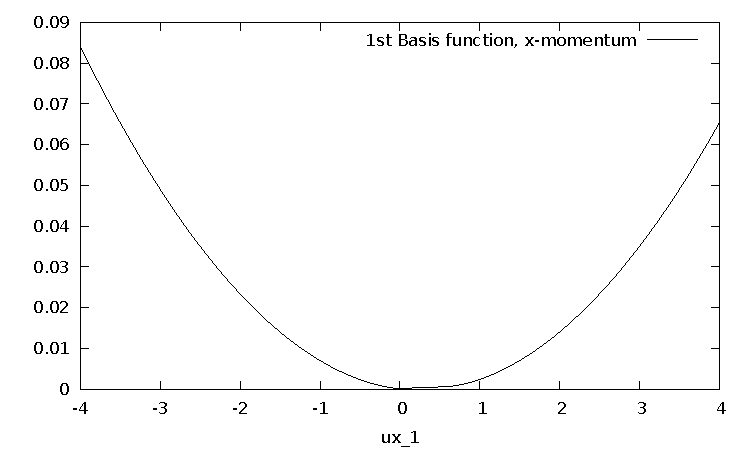
\includegraphics[scale=\zoomfactor]{{{ord2_varying_ux1_uy2_1/10.0_10.0_10.0_10.0_10.0_10.0_y_0.0_0.0_0.0_0.0_0.0_0.0_1.0_0.0_0.0_0.0_0.0f00}}}
  }
  \subfigure[2nd basis function, $x$-momentum] {
    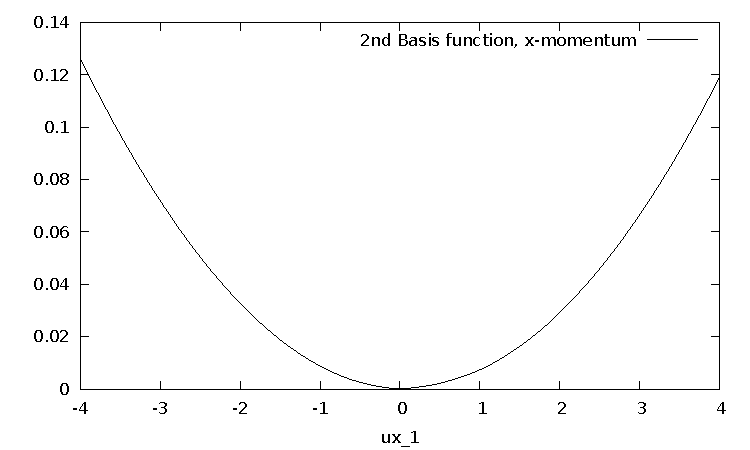
\includegraphics[scale=\zoomfactor]{{{ord2_varying_ux1_uy2_1/10.0_10.0_10.0_10.0_10.0_10.0_y_0.0_0.0_0.0_0.0_0.0_0.0_1.0_0.0_0.0_0.0_0.0f02}}}
  }
  \subfigure[3rd basis function, $x$-momentum] {
    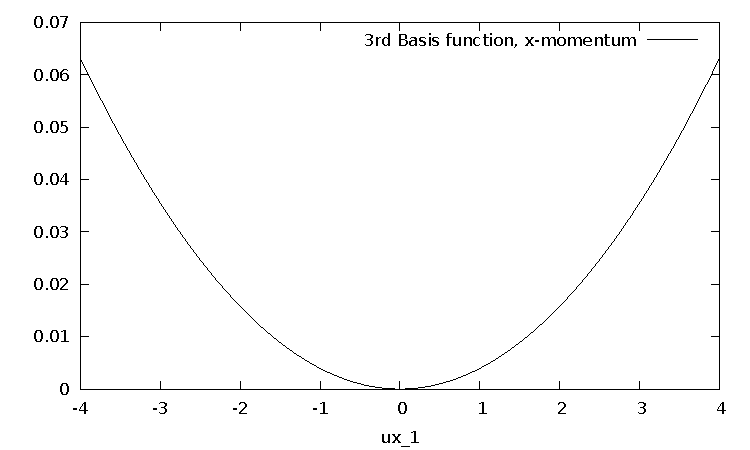
\includegraphics[scale=\zoomfactor]{{{ord2_varying_ux1_uy2_1/10.0_10.0_10.0_10.0_10.0_10.0_y_0.0_0.0_0.0_0.0_0.0_0.0_1.0_0.0_0.0_0.0_0.0f04}}}
  }
  \subfigure[4th basis function, $x$-momentum] {
    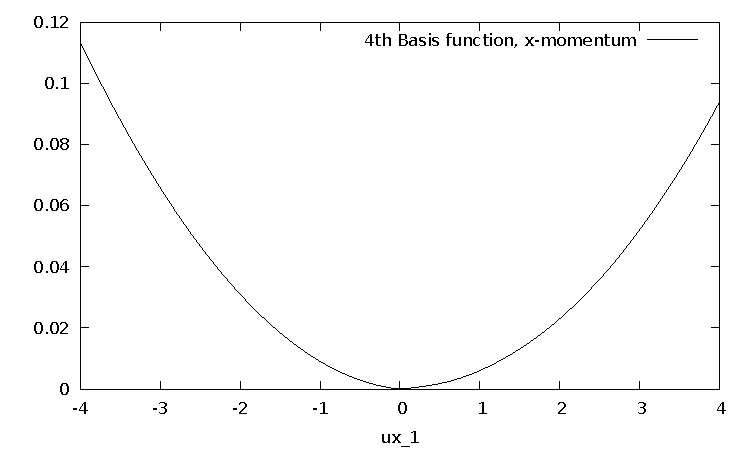
\includegraphics[scale=\zoomfactor]{{{ord2_varying_ux1_uy2_1/10.0_10.0_10.0_10.0_10.0_10.0_y_0.0_0.0_0.0_0.0_0.0_0.0_1.0_0.0_0.0_0.0_0.0f06}}}
  }
  \subfigure[5th basis function, $x$-momentum] {
    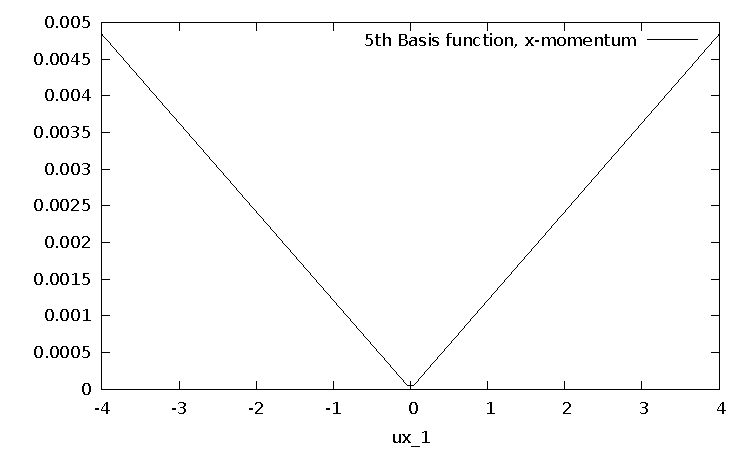
\includegraphics[scale=\zoomfactor]{{{ord2_varying_ux1_uy2_1/10.0_10.0_10.0_10.0_10.0_10.0_y_0.0_0.0_0.0_0.0_0.0_0.0_1.0_0.0_0.0_0.0_0.0f08}}}
  }
  \subfigure[6th basis function, $x$-momentum] {
    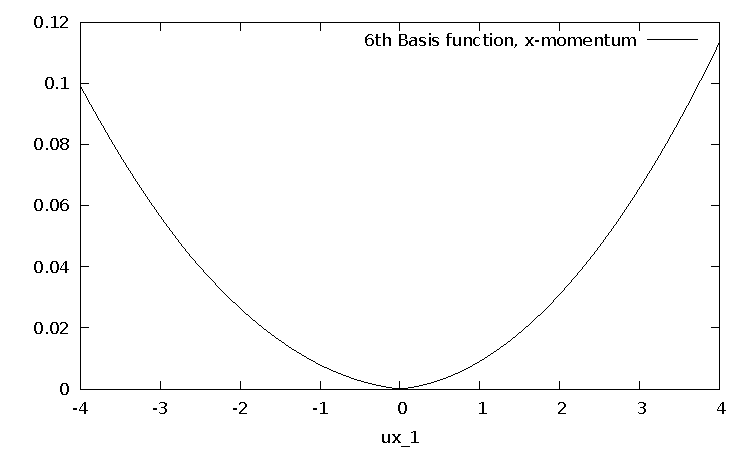
\includegraphics[scale=\zoomfactor]{{{ord2_varying_ux1_uy2_1/10.0_10.0_10.0_10.0_10.0_10.0_y_0.0_0.0_0.0_0.0_0.0_0.0_1.0_0.0_0.0_0.0_0.0f10}}}
  }
\caption{Error plots for $x$-momentums. All heights are 10, and all momentums except $u_{x,1}$ and $u_{y,2}$ are fixed to 0. The value $u_{y,2}$ is set to 1.}
\label{fig:ord2_varying_ux1_uy2_1}
\end{figure}

%%% Local Variables:
%%% TeX-master: "../results.tex"
%%% End:
